\documentclass[11pt, oneside]{article}   	% use "amsart" instead of "article" for AMSLaTeX format
\usepackage{geometry}                		% See geometry.pdf to learn the layout options. There are lots.
\geometry{letterpaper}                   		% ... or a4paper or a5paper or ... 
%\geometry{landscape}                		% Activate for for rotated page geometry
%\usepackage[parfill]{parskip}    		% Activate to begin paragraphs with an empty line rather than an indent
\usepackage{graphicx}				% Use pdf, png, jpg, or eps§ with pdflatex; use eps in DVI mode
								% TeX will automatically convert eps --> pdf in pdflatex		
\usepackage{amssymb}

\title{TestMine: Mining test evolution for improved software testing}
\author{Wasif Afzal}
\date{}							% Activate to display a given date or no date

\begin{document}
\maketitle
\section{Introduction}
There is an increasing reliance on software in our daily activities. This reliance mandates that software is able to meet its users' expectations, otherwise the consequences can be undesirable. During software development a range of verification and validation (V\&V) activities are performed with the goal of developing software that meets its requirements. Software testing is one major V\&V activity which aims to find \textit{as many defects as possible, as early as possible in the development phase, under given constraints of cost and schedule}~\cite{29119}. Clearly this is a challenging task, simply because there are not enough resources to test a software exhaustively. As a result, a lot of research has been done to make software testing efficient and effective. 

Software testing is typically performed at different levels, namely unit/component, integration, system and acceptance test levels. Also testing is performed as part of a specific life cycle model; agile development being the latest model. In agile, as the software is built incrementally, testing has to be a continuous process that needs to adapt with the changing nature of requirements. Issues such as timely identification of integration and regression issues and efficient system testing becomes critical concerns in an increment. Figure~\ref{fig:agile_incr} shows an example of how testing is an integrated part of an agile increment. 

\begin{figure} [h]
   \centering
   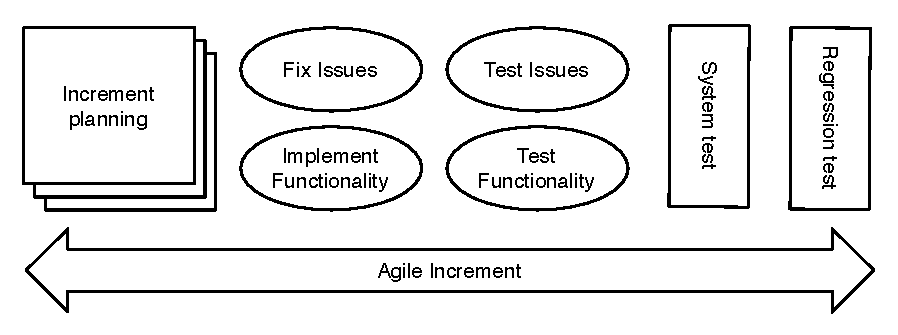
\includegraphics[width=80mm,height=35mm]{agile_incr.pdf}
   \caption{Testing in an agile increment (adapted from~\cite{29119}).}
   \label{fig:agile_incr}
\end{figure}

In agile the iterations are short, e.g., in Scrum each sprint is typically lasting one and four weeks. With the addition of new functionality and continuous fixing of issues in an increment (Figure~\ref{fig:agile_incr}), regression testing has to be done at its best. According to Engstr\"{o}m et al.~\cite{Emelie10}, iterative development strategies require frequent retesting of previously tested functions due to changes in related code and therefore it is important to use regression strategies that are efficient. As the number of increments increase, typically the regression test suite grows in size and becomes more expensive to run in each increment. This means that re-running every test case in the test suite will be expensive. This approach is generally called as \textit{retest all} and is the simplest regression test strategy~\cite{Graves01}. It is than natural to think about regression test selection (RTS) techniques as part of the overall regression test strategy. 

RTS techniques select subset of test cases from the test suite. It differs from test suite minimization or test suite reduction problem in the sense that it is modification-aware, i.e., the selection is specific to the current version of the program and is focussed on the modified parts of the program~\cite{Yoo12}. RTS thus verifies the behaviour of modified software. More formally, given an initial program \textit{P}, an original test suite \textit{T} associated with \textit{P} and a modified version of the program \textit{P'}, RTS techniques find a subset of \textit{T}, \textit{T'} to test \textit{P'}. 

RTS techniques have its own share of challenges. Such techniques can be costly to run and can miss potentially fault revealing test cases. Therefore it is always a trade-off between time required to select and run test cases and the fault detection ability of test cases~\cite{Graves01}. This trade-off is also highlighted by Engstr\"{o}m et al.~\cite{Emelie10}: \textit{[\ldots] there is a trade-off between cost reduction and defect detection ability. This is the case in all test selections, and none of the evaluated techniques seems to have done any major breakthrough in solving this trade-off.}

There are different classification schemes for RTS techniques but the most used classification property is whether these techniques are \textit{safe} or \textit{unsafe}~\cite{Emelie10}. A safe RTS technique ensures that the test suite \textit{T'} has all tests in \textit{T} that execute code that was changed from \textit{P} to \textit{P'}~\cite{Harrold99}. So with safe RTS techniques the faults found with tests in \textit{T} are also found with tests in \textit{T'}~\cite{Emelie10}. Harrold~\cite{Harrold99} calls such tests as \textit{modification traversing} for \textit{P} and \textit{P'}.  In other words if there is a modification traversing test case in the test suite, it will definitely be selected by a safe RTS technique~\cite{Yoo12}. However Rothermel and Harrold~\cite{Rothermel96} shows that precisely identifying modification traversing tests in T is difficult in practice due to non-determinism in programs and test execution, e.g., testing of a system ported to different operating system. As a result, several RTS techniques can be found in literature with varying precision and efficiency. This, again, helps explain the trade-off that exists in RTS techniques between cost and defect detection effectiveness. An unsafe RTS technique is one that may miss tests from \textit{T'} that are modification traversing. An unsafe RTS technique may be beneficial in cases where parts of \textit{P'} remain untested (or not covered) after running \textit{T'}. A simple example of unsafe RTS technique is random selection of test cases~\cite{Emelie10}. 

Apart from the safe-unsafe classification, Yu et al.~\cite{Yu12} presents another interesting multidimensional way to classify (safe) RTS techniques in terms of \textit{software}, \textit{bug} and \textit{data} dimensions. Within the \textit{software} dimension, the two most important research directions are categorised as \textit{code-based} and \textit{model-based} approaches. In deed most of the RTS research falls in the software dimension where techniques operate at different granularity levels; Orso et al.~\cite{Orso04} differentiates between techniques operating at high-level (such as at the method or class level) and those operating at low-level (such as at the level of statements). This is to say that a large body of literature on RTS techniques analyse code, at different abstraction levels, to seek modifications in the program under test. The model-based approaches represent a departure from source code being an input to having other software artefacts, such as activity diagrams and other UML based design documents.

%\subsection{}

\bibliographystyle{abbrv}
\bibliography{untitled}   % references.bib


\end{document}  